\section{Materials and Methods}
\label{sec:materials_methods}

\subsection{Study Area and Regional Landscape Characterization}
\label{subsec:study_area}

The investigation covers the entire province of Central Kalimantan, Indonesia, extending between latitudes 0.8$^\circ$\,N to 3.6$^\circ$\,S and longitudes 110.7$^\circ$\,E to 115.9$^\circ$\,E, covering approximately 153,564\,km$^2$ (Figure~\ref{fig:study_area}a). The province is partitioned administratively into 13 regencies and one autonomous urban municipality (Palangka Raya City), structured into five spatial cross-validation blocks (Figure~\ref{fig:study_area}b). Geomorphologically, Central Kalimantan exhibits a pronounced north-to-south gradient: the northern interior comprises rugged upland terrain defined by the Schwaner and M{\"u}ller mountain ranges situated on mineral soils and covered by primary and secondary dipterocarp rainforests. Conversely, the central and southern sectors form vast alluvial lowlands and ombrotrophic peat swamp basins drained by nine principal south-flowing rivers: the Jelai, Kumai, Seruyan, Mentaya, Katingan, Sebangau, Kahayan, Kapuas, and Barito rivers.

The southern peatland belt houses the historic Mega Rice Project (ex-PLG) footprint, which was excavated during 1995--1999 across four major planning blocks (Figure~\ref{fig:study_area}c):
\begin{itemize}
    \item \textbf{Block A} ($\sim$300,000\,ha): Flanked by the Kapuas and Barito rivers, centered within the Kapuas Regency (Mentangai, Dadahup, and Jenamas districts).
    \item \textbf{Block B} ($\sim$160,000\,ha): Located between the Kahayan and Kapuas rivers, centered in the Pulang Pisau Regency (Jabiren, Basarang, and Kahayan Hilir districts).
    \item \textbf{Block C} ($\sim$390,000\,ha): Situated between the Sebangau and Kahayan rivers, encompassing the southern peat outskirts of Palangka Raya City (Kalampangan, Bereng Bengkel) and northern Pulang Pisau.
    \item \textbf{Block D} ($\sim$150,000\,ha): Encompassing the coastal peat dome south of the Kahayan river extending toward Sebangau Kuala.
\end{itemize}

\clearpage

\begin{figure}[t!]
\centering
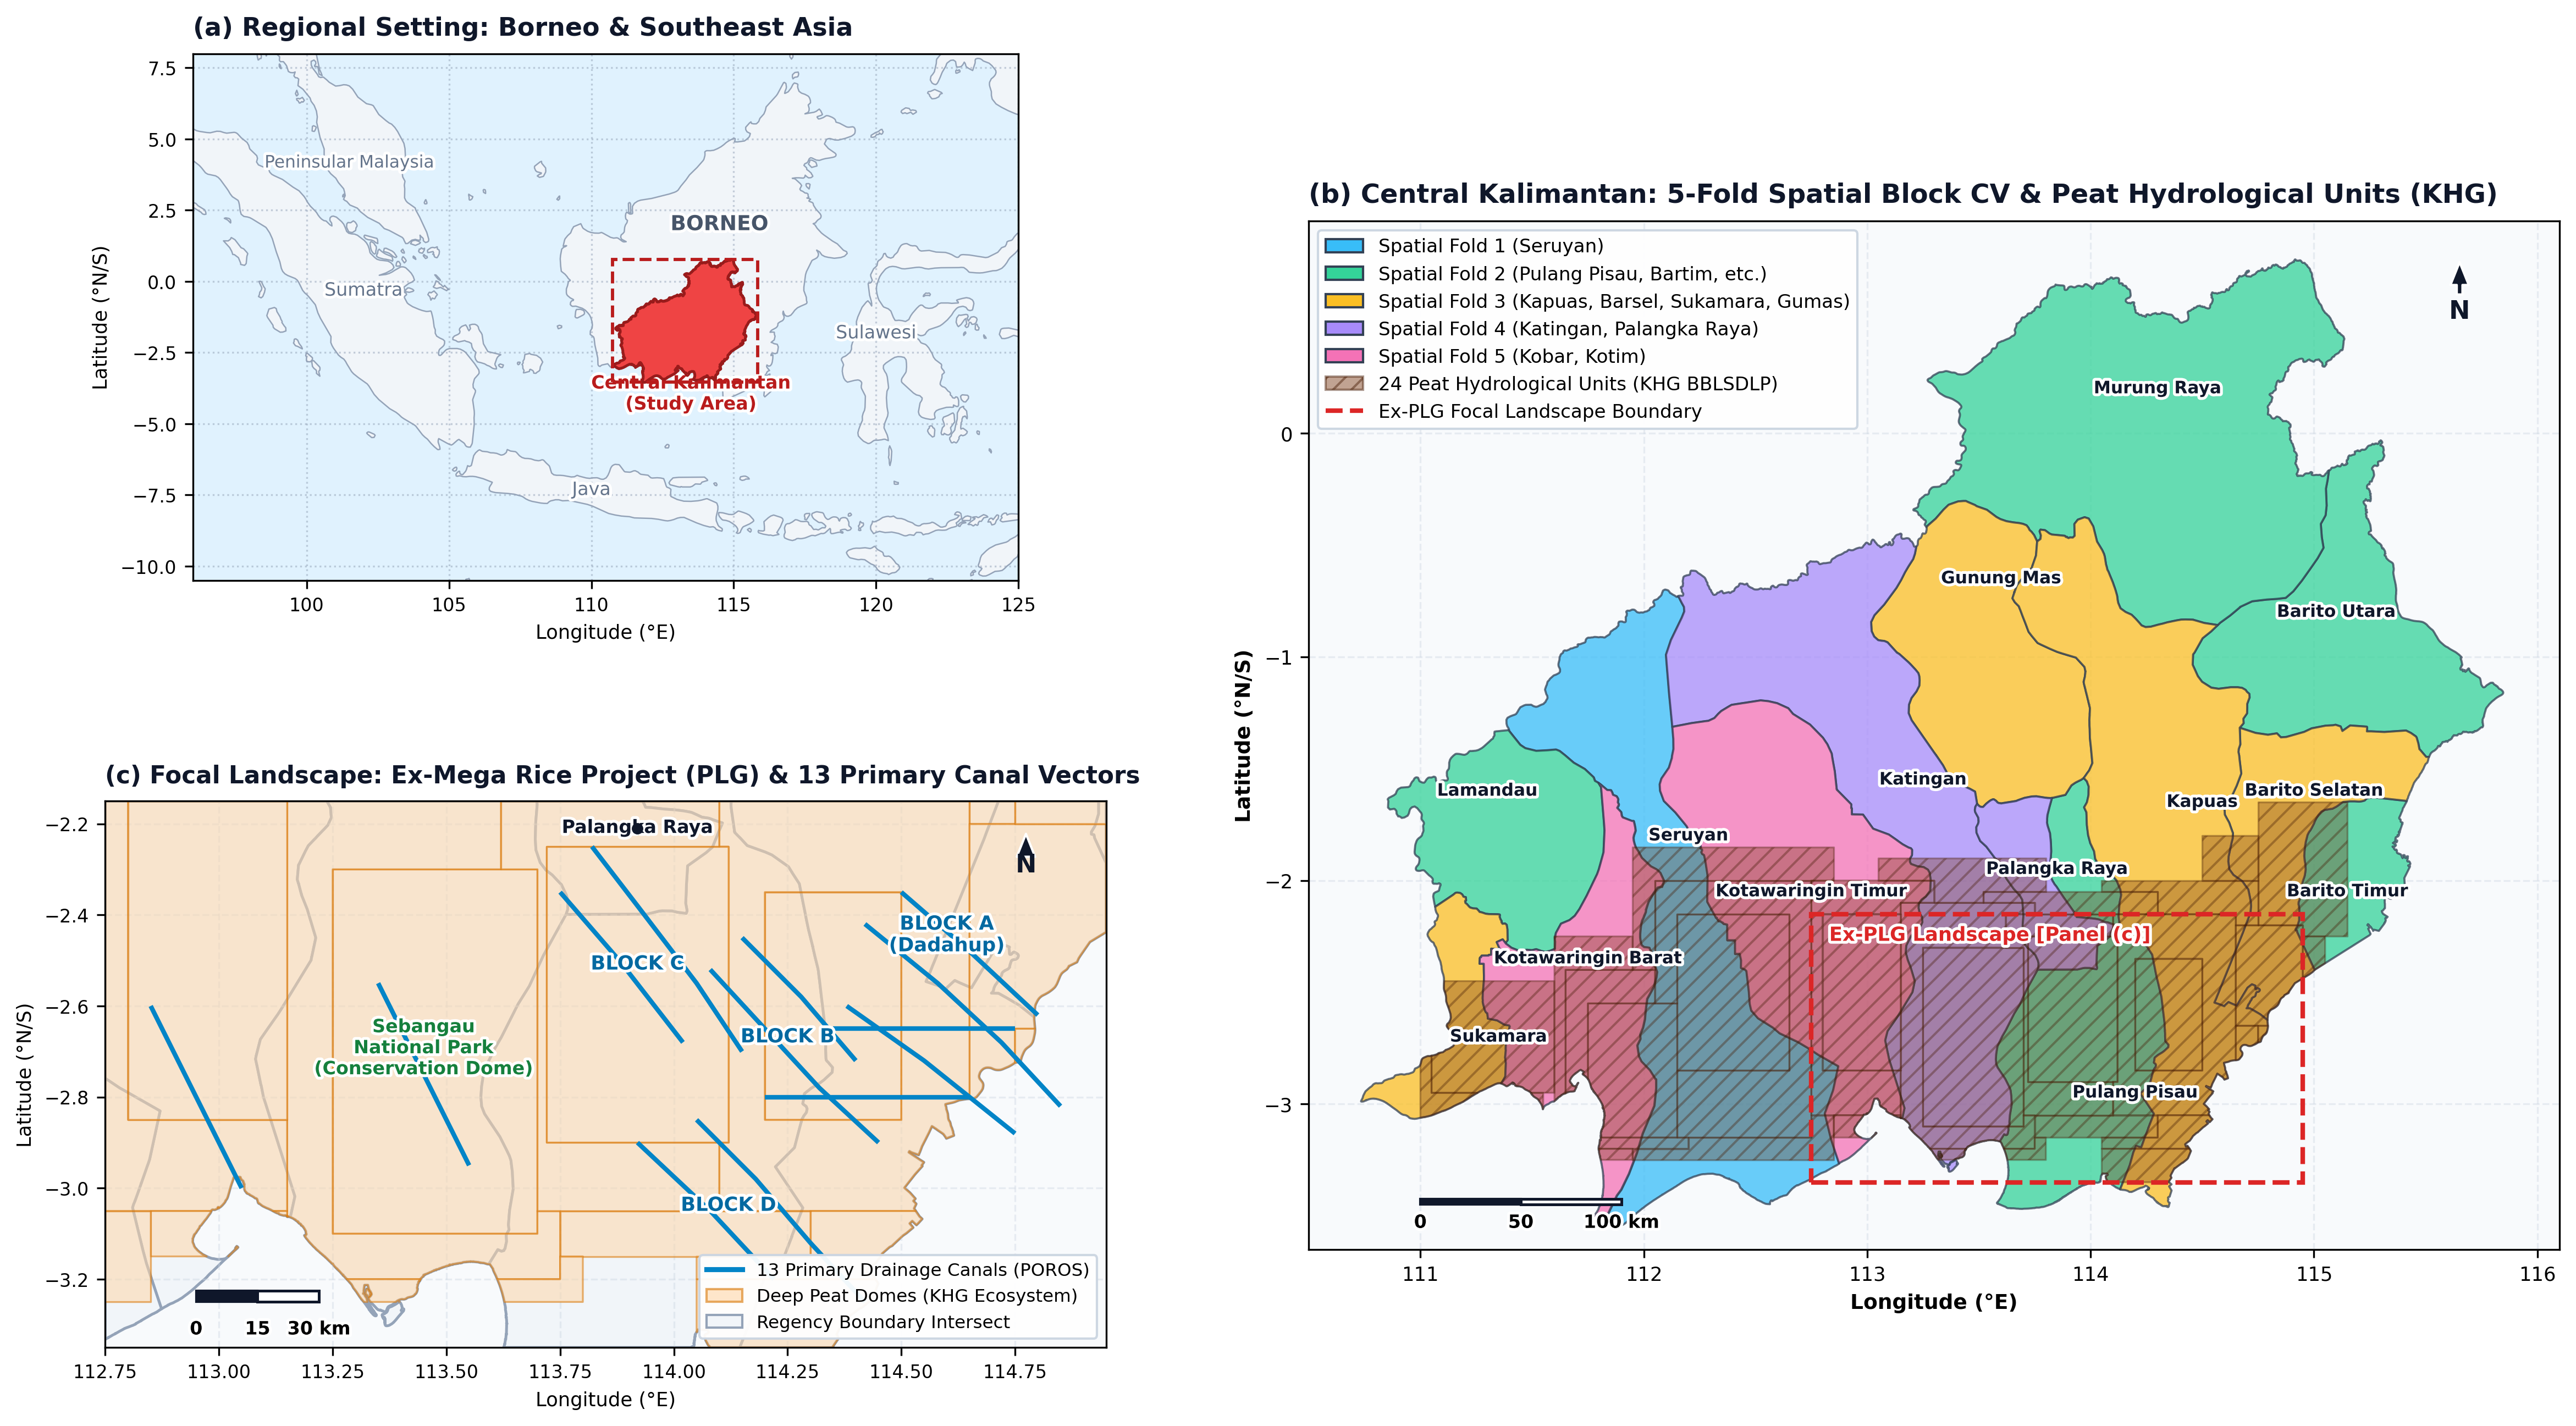
\includegraphics[width=0.88\textwidth]{01_peta_wilayah_studi_spatial_cv.png}
\caption{\textbf{Geographic setting, spatial cross-validation partitioning, and degraded peatland infrastructure in Central Kalimantan, Indonesia.} \textbf{(a)} Regional inset showing the geographic position of Central Kalimantan within Borneo Island and Maritime Southeast Asia. \textbf{(b)} Provincial cartography featuring all 14 regencies and municipalities classified into five Spatial Block Cross-Validation partitions (\texttt{GroupKFold}), overlaid with the 24 official Peat Hydrological Units (KHG) from the BBLSDLP database. \textbf{(c)} Focal landscape zoom of the ex-Mega Rice Project (ex-PLG) peatland territory (Blocks A, B, C, and D) delineating the 13 primary drainage canal vectors (Saluran Primer Induk / SPI), Sebangau National Park conservation dome, metric scale bar, and cartographic graticules.}
\label{fig:study_area}
\end{figure}

\subsection{Multisource Geospatial Data Ingestion and Processing Pipeline}
\label{subsec:data_pipeline}

\subsubsection{Active Fire Remote Sensing (NASA FIRMS)}
\label{subsubsec:firms_data}

Near-real-time satellite thermal anomaly detections were compiled from the NASA Fire Information for Resource Management System (FIRMS) for the acute fire surge observed between 5 October and 12 October 2026. The data stream combined observations from three polar-orbiting satellite sensor configurations:
\begin{enumerate}
    \item \textbf{VIIRS on Suomi-NPP}: 375\,m nominal spatial resolution in the I-band ($3.74$--$3.93\,\mu\text{m}$), providing daytime and nighttime passes \citep{Schroeder2021RSE, Roberts2020RS}.
    \item \textbf{VIIRS on NOAA-20}: Identical 375\,m I-band sensor configuration operating on a sun-synchronous orbit offset by approximately 50 minutes \citep{Schroeder2021RSE}.
    \item \textbf{MODIS on Aqua}: 1\,km spatial resolution (Collection 6.1 active fire algorithm) operating with daytime overpass at $\sim$13:30 local solar time \citep{Giglio2020RSE}.
\end{enumerate}

Initial provincial bounding box extraction yielded 52,829 raw candidate thermal detections. To eliminate boundary contamination from adjacent provinces (West Kalimantan and South Kalimantan) and discard peripheral edge artifacts, we performed an automated spatial point-in-polygon clipping operation using official high-resolution administrative boundary vectors (geoBoundaries ADM2, 14 provincial units). This spatial filter excluded 8,892 out-of-boundary observations (16.83\%), yielding 43,937 verified active fire hotspots located within Central Kalimantan.

Recorded attributes for each hotspot include acquisition date (\texttt{acq\_date}), UTC acquisition timestamp (\texttt{acq\_time}), geodetic coordinates (\texttt{latitude}, \texttt{longitude}), sensor instrument (\texttt{satellite}), algorithmic detection confidence (\texttt{confidence}), mid-infrared brightness temperature in kelvins (\texttt{brightness\_k}), and Fire Radiative Power in megawatts (\texttt{frp\_mw}) \citep{Roberts2015RSE, Chuvieco2019ESSD}.

\subsubsection{Peatland Delineation and Depth Stratification}
\label{subsubsec:peat_depth}

Peatland spatial boundaries and depth classifications were obtained from the official national peatland database compiled by the Indonesian Center for Agricultural Land Resources Research and Development (BBLSDLP, Ministry of Agriculture, 2019) and the Ministry of Environment and Forestry (Decree SK.130/MENLHK/SETJEN/PKL.0/2/2017 delineating the National Peat Hydrological Units / KHG). The vector database delineates 24 distinct peat dome units in Central Kalimantan across five standardized depth strata:
\begin{enumerate}
    \item \textbf{Shallow Peat} (50--100\,cm depth; median baseline: 75\,cm).
    \item \textbf{Medium Peat} (100--200\,cm depth; median baseline: 150\,cm).
    \item \textbf{Deep Peat} (200--300\,cm depth; median baseline: 250\,cm).
    \item \textbf{Very Deep Peat} ($>300$\,cm depth; median baseline: 390\,cm).
    \item \textbf{Mineral Soil} (\textit{Tanah Mineral}, non-peat mineral formations, assigned depth: 0\,cm).
\end{enumerate}
Each FIRMS hotspot was intersected against this polygon database. Detections located outside delineated peat polygons were classified as Mineral Soil with a peat depth of 0\,cm.

\subsubsection{Canal Vector Network and Projected Metric Drainage Distance}
\label{subsubsec:canal_network}

To quantify the hydrological drainage impact of artificial canals without geodetic distortion, the primary canal backbone (Saluran Primer Induk / SPI) of the Mega Rice Project Blocks A, B, C, and D was vectorized as a multi-segment line network comprising 13 primary canal axes.

Both active fire coordinates and canal polyline vectors were reprojected from WGS~84 geographic coordinates (EPSG:4326) into the official metric projected coordinate system for Central Kalimantan, \textbf{WGS~84 / UTM Zone 49S} (\mbox{EPSG:32749}). The minimum Euclidean distance from each hotspot to the nearest primary canal line was computed according to Equation~\eqref{eq:canal_dist}:
\begin{equation}
d_{\text{canal}, i} = \min_{j \in \{1, \dots, M\}} \left\| \mathbf{p}_i - \mathbf{c}_j \right\|_2 = \min_{j} \sqrt{(x_i - u_j)^2 + (y_i - v_j)^2}
\label{eq:canal_dist}
\end{equation}
where $\mathbf{p}_i = (x_i, y_i)$ represents the projected UTM Zone 49S coordinates (in meters) of hotspot $i$, and $\mathbf{c}_j = (u_j, v_j)$ represents the vertices of primary canal vector segments.

To prevent geographic distortion in western regencies that do not contain ex-PLG canal networks (e.g., Seruyan, Kotawaringin Barat, Kotawaringin Timur), a binary landscape zoning indicator was established as formulated in Equation~\eqref{eq:ex_plg}:
\begin{equation}
\text{is\_ex\_plg\_landscape} = \begin{cases} 
1, & \text{if Regency} \in \{\text{Pulang Pisau, Kapuas, Palangka Raya City}\} \\ 
0, & \text{otherwise} 
\end{cases}
\label{eq:ex_plg}
\end{equation}
For hotspots outside the ex-PLG landscape, the operational canal distance feature was assigned a standardized sentinel value of $-1$, whereas points within the ex-PLG zone retained their true Euclidean drainage proximity in meters. This prevents spurious distance measurements to distant canals that exert zero hydrological influence over western peat domes.

\subsubsection{Atmospheric Reanalysis and Fire Weather Modeling}
\label{subsubsec:weather_era5}

Daily atmospheric forcing data were obtained from the European Centre for Medium-Range Weather Forecasts (ECMWF) ERA5-Land atmospheric reanalysis dataset (nominal horizontal grid resolution of $0.1^\circ \approx 9$\,km). Reanalysis variables were compiled across all 14 administrative centroids for a 30-day antecedent window prior to each fire observation. Extracted daily meteorological indicators include:
\begin{itemize}
    \item Maximum 2-meter air temperature ($T_{\text{max}}$, $^\circ\text{C}$).
    \item Mean 2-meter relative humidity ($\text{RH}_{\text{mean}}$, \%).
    \item Maximum 10-meter horizontal wind speed ($W_{\text{max}}$, km/h).
    \item Daily precipitation ($P_{\text{daily}}$, mm).
    \item 7-day cumulative antecedent precipitation ($P_{\text{7d}} = \sum_{t=0}^{6} P_{t}$, mm).
    \item 14-day cumulative antecedent precipitation ($P_{\text{14d}} = \sum_{t=0}^{13} P_{t}$, mm).
    \item Consecutive dry spell duration ($D_{\text{spell}}$, days with $P_{\text{daily}} < 1.0$\,mm).
\end{itemize}

A regionally calibrated Fire Weather Index ($\text{FWI}$) was formulated following the Canadian Forest Fire Weather Index / BMKG Fire Danger Rating framework adapted for tropical peat environments (Equation~\eqref{eq:fwi}) \citep{Spessa2015Biogeosciences}:
\begin{equation}
\text{FWI}_i = 0.35\,T_{\text{max}, i} + 1.35\,D_{\text{spell}, i} - 0.22\,P_{\text{7d}, i} + 0.22\,(100 - \text{RH}_{\text{mean}, i}) + 0.25\,W_{\text{max}, i}
\label{eq:fwi}
\end{equation}

\subsubsection{Cadastral Land Tenure Overlay}
\label{subsubsec:tenure_overlay}

To evaluate land tenure attribution, official concession boundary shapefiles were obtained from the national cadastral registry:
\begin{enumerate}
    \item \textbf{Oil Palm Plantations}: 627 certified Right to Cultivate (HGU) corporate concession polygons administered by the National Land Agency (BPN).
    \item \textbf{Commercial Forestry Concessions}: 185 Forest Utilization Business License (PBPH) polygons issued by the Ministry of Environment and Forestry (KLHK).
\end{enumerate}

Through automated spatial overlay, each active fire observation was classified into one of three mutually exclusive legal tenure categories:
\begin{itemize}
    \item \textbf{Oil Palm Concessions (HGU)} (\texttt{concession\_oil\_palm}): Hotspots located within certified corporate oil palm concession boundaries.
    \item \textbf{Commercial Forestry Concessions (PBPH)} (\texttt{concession\_forestry}): Hotspots located within commercial timber or ecosystem restoration forestry concessions.
    \item \textbf{Non-Concession Land (APL)} (\texttt{non\_concession\_apl}): Hotspots located outside concessions on state Other Utilization Areas (APL), community agroforestry lands, or unallocated degraded peatlands \citep{Putranto2023LandUsePol}.
\end{itemize}

A comprehensive summary of all feature variables ingested into the predictive modeling pipeline is presented in Table~\ref{tab:feature_inventory}.

\begin{table}[htbp]
\centering
\caption{\textbf{Inventory of geospatial, meteorological, edaphic, and tenurial features compiled for active fire intensity modeling in Central Kalimantan.}}
\label{tab:feature_inventory}
\small
\begin{tabularx}{\textwidth}{lllLP{3.0cm}}
\toprule
\textbf{Feature Identifier} & \textbf{Type} & \textbf{Units} & \textbf{Biophysical / Governance Description} & \textbf{Data Source} \\
\midrule
\texttt{frp\_mw} & Continuous & MW & Fire Radiative Power (intensity target proxy) & NASA FIRMS \\
\texttt{target\_extreme} ($y$) & Binary & $\{0, 1\}$ & Severe fire indicator ($\text{FRP} \ge 12.0$\,MW) & Target variable \\
\texttt{latitude} & Continuous & Decimal deg. & Geodetic north-south coordinate (Model~A only) & NASA FIRMS \\
\texttt{longitude} & Continuous & Decimal deg. & Geodetic east-west coordinate (Model~A only) & NASA FIRMS \\
\texttt{regency\_name} & Categorical & String & Administrative regency identifier (Model~A only) & geoBoundaries \\
\texttt{canal\_distance\_m} & Continuous & Meters & UTM Zone 49S Euclidean distance to canal ($d_{\text{canal}}$) & Mega Rice Project vector \\
\texttt{is\_ex\_plg} & Binary & $\{0, 1\}$ & Indicator for Mega Rice Project landscape corridor & Regional zoning \\
\texttt{peat\_depth\_cm} & Continuous & cm & Peat dome thickness ($d_{\text{peat}}$, 0 to 390\,cm) & BBLSDLP (2019) \\
\texttt{soil\_type} & Categorical & String & Edaphic soil class (Mineral vs. Shallow/Deep Peat) & BBLSDLP (2019) \\
\texttt{rainfall\_7d\_mm} & Continuous & mm & 7-day cumulative antecedent rainfall ($P_{\text{7d}}$) & ECMWF ERA5-Land \\
\texttt{rainfall\_14d\_mm} & Continuous & mm & 14-day cumulative antecedent rainfall ($P_{\text{14d}}$) & ECMWF ERA5-Land \\
\texttt{temp\_max\_c} & Continuous & $^\circ\text{C}$ & Maximum 2-meter daily air temperature ($T_{\text{max}}$) & ECMWF ERA5-Land \\
\texttt{relative\_humidity} & Continuous & \% & Mean 2-meter relative air humidity ($\text{RH}_{\text{mean}}$) & ECMWF ERA5-Land \\
\texttt{wind\_speed\_kmh} & Continuous & km/h & Maximum 10-meter horizontal wind speed ($W_{\text{max}}$) & ECMWF ERA5-Land \\
\texttt{dry\_spell\_days} & Integer & Days & Consecutive dry spell duration ($D_{\text{spell}}$) & ECMWF ERA5-Land \\
\texttt{fwi\_score} & Continuous & Index & Fire Weather Index composite risk score & Calibrated formulation \\
\texttt{land\_cover} & Categorical & String & Vegetation land cover class (shrub, forest, etc.) & KLHK Land Cover \\
\texttt{concession\_status} & Categorical & String & Cadastral tenure status (APL vs. HGU vs. PBPH) & BPN \& KLHK Cadastre \\
\bottomrule
\end{tabularx}
\end{table}

\subsection{Predictive Machine Learning and Validation Framework}
\label{subsec:ml_framework}

\subsubsection{Target Formulation: Severe Fire Radiative Power}
\label{subsubsec:target_def}

Conventional wildfire machine learning models frequently configure a binary presence-absence task against randomly sampled pseudo-absences. In this investigation, we model the intensity of ignited fires to differentiate moderate surface burning from severe, high-energy radiative events capable of sustaining deep subterranean peat smoldering.

Following calibration thresholds for satellite infrared sensors over tropical biomass \citep{RobertsWooster2008JGR, Wooster2018NatGeosci}, the binary classification target $y_i$ is formulated as defined in Equation~\eqref{eq:target}:
\begin{equation}
y_i = \begin{cases} 
1, & \text{if } \text{FRP}_i \ge 12.0\text{ MW (Severe / High-Energy Radiative Fire)} \\ 
0, & \text{if } \text{FRP}_i < 12.0\text{ MW (Regular / Moderate Incipient Fire)} 
\end{cases}
\label{eq:target}
\end{equation}
Within the 43,937 verified observations, 6,648 detections (15.13\%) were classified as severe fires ($y=1$), while 37,289 detections (84.87\%) represented regular fires ($y=0$), establishing an empirical class imbalance ratio of approximately $1 : 5.6$.

To prevent the machine learning algorithm from optimizing majority-class accuracy at the expense of severe fire sensitivity, we applied an inverse class weighting strategy (Equation~\eqref{eq:class_weight}):
\begin{equation}
w_c = \frac{N}{K \cdot n_c}
\label{eq:class_weight}
\end{equation}
where $N = 43,937$, $K = 2$, $n_1 = 6,648$ (severe class), and $n_0 = 37,289$ (regular class). This yielded class weights of $w_1 \approx 3.3045$ and $w_0 \approx 0.5891$, imposing a 5.6-fold higher penalty on false-negative misclassifications of severe fire events.

\subsubsection{Comparative Architectures: Model A vs. Model B}
\label{subsubsec:model_architectures}

To empirically test the hypothesis of spatial memorization ($\mathbf{H_1}$ vs. $\mathbf{H_2}$), we formulated two distinct Random Forest classifier pipelines \citep{Breiman2001ML}:
\begin{itemize}
    \item Model A (Spatial Memorization): 15 predictors (Equation~\eqref{eq:features_a}), including geodetic coordinates and regency identifiers:
    \begin{equation}
    \begin{aligned}
    \mathbf{X}_A = \{ & \text{lat}, \text{lon}, \text{regency}, d_{\text{canal}}, \text{is\_ex\_plg}, d_{\text{peat}}, P_{\text{7d}}, T_{\text{max}}, \\
    & \text{RH}, W_{\text{max}}, D_{\text{spell}}, \text{FWI}, \text{soil\_type}, \text{cover\_type}, \text{tenure} \}
    \end{aligned}
    \label{eq:features_a}
    \end{equation}
    \item Model B (Pure Biophysical Model): 12 environmental, hydrological, and tenurial predictors (Equation~\eqref{eq:features_b}), without spatial coordinates or administrative identifiers:
    \begin{equation}
    \begin{aligned}
    \mathbf{X}_B = \{ & d_{\text{canal}}, \text{is\_ex\_plg}, d_{\text{peat}}, P_{\text{7d}}, T_{\text{max}}, \text{RH}, \\
    & W_{\text{max}}, D_{\text{spell}}, \text{FWI}, \text{soil\_type}, \text{cover\_type}, \text{tenure} \}
    \end{aligned}
    \label{eq:features_b}
    \end{equation}
\end{itemize}

Hyperparameter configurations were held constant across both pipelines to ensure strict comparability: number of estimators $n_{\text{estimators}} = 150$, maximum tree depth $\text{max\_depth} = 10$, minimum samples per split $\text{min\_samples\_split} = 6$, and `\texttt{class\_weight=balanced}'.

\subsubsection{Spatial Block Cross-Validation Protocol}
\label{subsubsec:spatial_cv_protocol}

Both models were subjected to two evaluation regimes:
\begin{enumerate}
    \item \textbf{Stratified Random Holdout Split (75:25)}: A standard benchmark splitting the dataset randomly while preserving target proportions ($n_{\text{train}} = 32,952$; $n_{\text{test}} = 10,985$).
    \item \textbf{Spatial Block Cross-Validation (\texttt{GroupKFold}, $K=5$)}: A spatial partitioning protocol where the entire dataset $\mathcal{D}$ is partitioned into five mutually exclusive geographical blocks grouped by regency (Equation~\eqref{eq:spatial_cv}):
    \begin{equation}
    \mathcal{D} = \bigcup_{k=1}^{K} \mathcal{D}_k, \quad \mathcal{D}_k \cap \mathcal{D}_l = \emptyset \quad \forall k \ne l
    \label{eq:spatial_cv}
    \end{equation}
    In each cross-validation fold $k$, the model is trained on $\mathcal{D}_{\text{train}} = \mathcal{D} \setminus \mathcal{D}_k$ and evaluated exclusively on held-out geographic units $\mathcal{D}_k$. The spatial block allocation grouped regencies as follows:
    \begin{itemize}
        \item \textbf{Fold 1}: Seruyan (western coastal peat dome complex).
        \item \textbf{Fold 2}: Pulang Pisau, Barito Timur, Barito Utara, Lamandau, Murung Raya.
        \item \textbf{Fold 3}: Kapuas, Barito Selatan, Gunung Mas, Sukamara.
        \item \textbf{Fold 4}: Katingan, Palangka Raya City.
        \item \textbf{Fold 5}: Kotawaringin Barat, Kotawaringin Timur.
    \end{itemize}
\end{enumerate}

Evaluation metrics computed across both regimes include Area Under the Receiver Operating Characteristic Curve (ROC-AUC), precision, recall, and $F_1$-score for both regular and severe fire categories.

\subsubsection{Explainable Artificial Intelligence: TreeSHAP Decomposition}
\label{subsubsec:treeshap}

To interpret the non-linear decision surface of the Pure Biophysical Model (Model~B), we computed exact Shapley values using the TreeSHAP algorithm \citep{LundbergLee2017NeurIPS}. For a tree ensemble prediction function $f(\mathbf{x})$, the Shapley attribution $\phi_j$ uniquely decomposes the difference between the local prediction and the expected background value $\mathbb{E}[f(\mathbf{X})]$ according to Equation~\eqref{eq:shap}:
\begin{equation}
f(\mathbf{x}) = \phi_0 + \sum_{j=1}^{M} \phi_j(\mathbf{x}), \quad \phi_j(f, \mathbf{x}) = \sum_{S \subseteq \mathcal{F} \setminus \{j\}} \frac{|S|!(|\mathcal{F}| - |S| - 1)!}{|\mathcal{F}|!} \left[ f(S \cup \{j\}) - f(S) \right]
\label{eq:shap}
\end{equation}
where $\mathcal{F}$ represents the full set of $M$ features, $S$ denotes feature subsets, and $\phi_0 = \mathbb{E}[f(\mathbf{X})]$. TreeSHAP values were computed across a stratified holdout sample of 2,500 observations for the severe fire class ($y=1$) to evaluate feature rankings and discover non-linear tipping points.
